\chapter{Sprint 1}
This chapter covers the work for the first sprint in the aStep project. Seeing as the project is new, the initial focus will be to research technologies and attempt an early design for the system. As such, the goals for this sprint is explore and possibly select technologies, as well as developing an initial design of the structure of the indoor positioning service. 

The following chapter describes the initial steps to integrate indoor positioning into aStep.

\section{System for Monitoring Mobile Devices}\label{sec:monitoring}\sfx{new name}
When monitoring electronic devices in indoor spaces, a set of obstacles are presented. Some of the popular techniques used in outdoor environments prove themselves obsolete or severely hindered when applied in an indoor environment. \sfx{source (Cant find it ask Anders - Oliver)} This can be seen when working with the Global Positioning System(GPS) technology, as obstacles such as walls, roofs and floors will disrupt the signals received from satellites, leading to large imprecisions in the position measurement. As a consequence we need to explore specialized methods for determining positions in indoor spaces.

In this section we will describe different approaches for indoor positioning and monitoring of mobile devices, and systems using these. Two systems will be described for indoor positioning, namely Google Indoor Maps and Cisco MSE.

\subsection{Tracking Approach}\label{sec:tracking_approach}
WI-FI, Bluetooth and Radio-Frequency Identification (RFID) are amongst the most popular technologies used for indoor positioning. When using these technologies there are multiple approaches for determining a users position. In this section we will examine some of these approaches.

Tracking approaches are typically mapped into four categories\cite{tracking_approaches}
\begin{itemize}
\item Cell of origin
\item Distance
\item Angle of Arrival
\item Location Patterning
\end{itemize}
Despite the division, many approaches combine categories to increase the location precision. We will take a look at an approach from each category.

\subsubsection*{Cell of Origin}
Approaches categorized under cell of origin are among the simplest techniques for positioning. These approaches aim to position mobile devices in cells, either defined by the reach of access points, or defined by rooms in a building.
The latter approach can utilise RFID to create checkpoints throughout a building. These checkpoint are placed in room entrances and consist of a RFID scanner, such that devices with a RFID tag are registered as they pass the scanner\cite{indoor_bin}. 
This approach can be used to track the RFID tags, as each tag contains a unique ID, which is combined with the RFID scanners ID and a time-stamp. By analysing the most recent entry, the system will be know in which room the tag is located\cite{RFIDjournal}.

The approaches in this category requires auxiliary hardware to set up the checkpoints, and is in addition to this limited to only work at these checkpoints. By analysing the collected data on the host system it is possible to track a device. Thereby it can be know if a device have entered or exited the room. It can however not know where in the room the device is, which makes it difficult to track someone if a room is of substantial size or the building lacks RFID scanners\cite{RFIDjournal}.

\subsubsection*{Distance}
%Triangulation
Approaches in the distance category measures the proximity of a device and use this information to calculate a position, much in the same way it is done by GPS.
Triangulation works by using three or more access-points to receive the signal from a device. The position of the access-points are known to the system and by calculating the distance from the device to each access-point, based on the Received Signal Strength Indication(RSSI), the position can be found \cite{Triangulation}. The RSSI can be used to measure proximity, using the fact that signal strength decays over distance. Naturally, the decay will be greater in a closed environment with disruptions for the signal, and as such signal loss models have been developed for indoor environments. 
\Cref{fig:triangulation} shows a simple model of how triangulation works. In the centre of each circle is a set of coordinates which is the position of the access-point. The circle indicates the proximity of the device. By using three access-points the exact position of the device can be resolved, by determining where the intersection of the three proximities is.
\begin{figure}[ht]
	\begin{center}
		\includegraphics[scale=1]{graphics/triangulation.png}
		\caption{Triangulation\cite{Triangulation}}
		\label{fig:triangulation}
	\end{center}
\end{figure}

\subsubsection*{Angle of Arrival}
This category consists of approaches where the angle of the received signal is measured. The angle can be obtained by either having several antennas or being able to rotate a single antenna to find the direction at which the RSSI is strongest. With multiple angles of arrival it is possible to calculate a position based on the intersection of the vectors going through the antennas.

\subsubsection*{Location Patterning}
The location patterning category sets out to measure the connectivity patterns for given locations. The most common approach for this category is called WI-FI Fingerprinting. It works by introducing an intial calibration phase, where the RSSI for each point of interest is measured and stored in the system. When the signal strength from a device is received, it is then compared to the previously measured RSSIs. The point of interest with the closest RSSI is determined to be the position of the device. This means that a system using fingerprinting can not determine the exact position of a device, but rather which area the device is currently at \cite{fingerprint1}.

\subsection{Evaluation dimensions}
When evaluating indoor location services there are three dimensions that have to be considered: location precision, refresh rate and system latency. Location precision tells us about the location precision that the system affords. Refresh rate is the rate at which the location is updated, and as such how closely the most recent data is related to real-time data. System latency is a dimension describing the time it takes to perform the positioning calculations\cite{dimensions}. Depending on the usage of the system, the dimensions can be valued using a scale of importance, such as "High", "Medium" and "Low". Alternatively we can chose to look for systems with one or more dimensions below a set value. For example, we have a desire to find a system with a location precision lower than the average precision for GPS. 

The three dimensions are in no way constant for a system. For most systems, the hardware has a large influence on the dimensions. Location precision is severely diminished if the environment lacks access points. Refresh rate depends on how often mobile devices communicate with the network and system latency can be impacted by a large amount of noise on the WI-FI channels. Naturally corporations developing indoor positioning services use their best results to advertise for their product. As such, the values supplied from official advertising sources are best-case values. However, if we assume this is the case for all products, we can use these values as a basis for comparison.

%What does google do?
\subsection{Technologies}
In this section we examine some systems that aStep can use to integrate indoor positioning.

Zonith Indoor Positioning System is a system that uses the Cell of Origin approach. As mentioned in \cref{sec:tracking_approach}, this technique requires auxiliary hardware. Zonith offers Bluetooth Beacons, which serve as checkpoint nodes, and allow for any device with Bluetooth to be discovered and tracked.
%http://zonith.com/products/ips/

Google presents one possible system. They have made indoor navigation and tracking possible trough their Indoor Maps project \cite{IPSoverGPS}, which lets users map a building by uploading a floor plan of said building. After the floor plan has been accepted, the system will request information about the location of the WI-FI access points in the building. By doing so, the system is able to triangulate using the access points as static reference points and combine that information with the GPS location, thereby utilising both technologies to get a more precise position of the device than by using GPS only.

%About Cisco
Cisco has developed a location-aware wireless network system, the Cisco Unified Wireless Network(UWN), which utilises WI-FI triangulation\cite{CiscoTri} and other wireless communication protocols in order to develop indoor location based services\cite{uwn}.
Cisco utilizes the Cisco Mobility Services Engine (MSE) for their system. The MSE makes it possible for Cisco to track the location of up to 25000 network devices at once. It is the MSE that does the calculations to position devices using the data it receives from the access-points\cite{ciscoMSE}.
The building is modelled by the use of an outline of the floor plan. The image will be converted to a coordinate system that is placed on top of the model which is then supplied with the positions of the access points that are set up in the building. From there it is possible to get the relative position of any nearby devices in relation to the origin of a coordinate system. It is these positions that will be used in order to track and analyse wireless devices.

\subsection{Choice of technology}\label{subsec:cisco}
Due to RFID not being able to position devices at any time, but is rather able to indicate where a device was last registered, it is not optimal for the applications currently being designed. It have therefore been chosen to use a WI-FI based system.
At the university we have access to a sever that runs the Cisco UWN (MSE) software, which is set up to monitor every building on campus at Aalborg University. We have chosen to use the data that is available from here as it is comprehensible to set the system up in a new environment.

%How do we solve the previous stated problems
%Alternative IPS 
%se what we did in cisco 
\section{Permission} \label{sec:permission}
By using Cisco it is possible to acquire and store peoples unique Mac-address and use this to track them. It is illegal to do so without the individuals acceptance and it is as such necessary to accommodate this regulation when designing the system \cite{TrafficIlligal}.
There have been several trials in Denmark as a consequence of this regulation. A Traffic system has recorded passerbys by registering the WI-FI signal emitted from their smart phones. This was done with sensors registering the unique Mac-address, which was then hashed and re-hashed in the sensors before being stored. Despite the attempt at obfuscating the users\cite{TrafficIlligal}, it is illegal according to the \textit{Directive on privacy and electronic communications} article 5(3)\cite{CookieDirective} which can be seen in the following quote,

\begin{quote}
\textit{'Member States shall ensure that the use of electronic communications networks to store information or to gain access to information stored in the terminal equipment of a subscriber or user is only allowed on condition that the subscriber or user concerned is provided with clear and comprehensive information...'}
\end{quote}

However, the Danish Business Authority's conclusion was that the system did not fit in \textit{Directive on privacy and electronic communications} due to the end-user being unidentifiable\cite{TrafficOK} as described by article 3(1)\cite{CookieDirective}. No sanction was inflicted for this case, however, as a consequence the system is no longer in use.

%http://eur-lex.europa.eu/legal-content/DA/TXT/PDF/?uri=CELEX:31995L0046&from=da
To ensure no such debates are raised in relation to this project, it will be necessary to differ between those who have given their permission to store person sensitive data and those who have not. By differentiating between the two it will be possible to obfuscate and remove personal data for individuals who has not given their acceptance.

We will use the term person sensitive data when referring to data that can be used to identify a person. 

\section{security}
The security aspect when working with the Cisco system will be minimized, because the security is not our main focus. This section will describe the requirements from working with sensitive data related to the Cisco system and how we handle these requirements.

The administrator for the Cisco system will only allow us to retrieve data, if we obfuscate the MAC-addresses and other sensitive data like email addresses, to protect personal data and prevent singling out a specific person without there permission. They also required that username and password would be necessary in order to establish connection. 

\subsection{Obfuscate MAC-Addresses}
There are several alternatives to obfuscate the MAC-address, we need a solution that allow us to still track the obfuscated MAC-address, this is done to not limit the capabilities of aSTEP indoor location based service. Our approach is to simply remove the last 4 digits of the MAC-address, the only exception is if user have agreed to let us save their MAC-address.
This is a simple solution that make sure the server does not store any sensitive data with the users accept. Long term goal for the aSTEP project is to incorporate security, so MAC-addresses is not stored in plain text, to raise security of the super project. This can also be seen in chapter \ref{Cha:Future_Work} about future work. 

%\subsubsection{Hashing}
%Hashing the MAC-address is a solution, the problem with that is the hash function takes an input and output into a fixed table, this can make two MAC-addresses share the same entry in the table, this can be fixed by expanding the hash function to cover all possible combinations of MAC-addresses and then eliminating the chance of two MAC-addresses have the same entry. This will make the table larger compared to the option were two MAC-addresses could have the same entry

%\subsubsection{Translating}
%A simpler approach that we suggested to the administrator of Cisco, is changing the last four digits of the MAC-address and replacing them with a counter, this will make it impossible to know which MAC-address corresponds to the real address. This was approved by the administrator.

%Hashing is a good option but more complex then simply translating the addresses, translations of MAC-address will be our chose over hashing.


%\subsection{Encryption}
%Encryption are used to ensured that only the intended people is able to extract data. Encrypting data is however not always enough, due to unauthorized people still being able to access the encrypted data and in practice be able to decrypt it. This can be semi-counteracted by increasing the bit encryption, which will exponentially increase the time needed to brute force the encryption. When security is discussed there are two impotent factors to consider. One: Two: \ofx{Source? and what are those two factors?}
\section{Using Cisco on AAU}
%husk at forklare om CPI og MSE
The Cisco localisation and positioning system is already in use on Aalborg University. To be able to use the information from the system, we had a meeting with the administrator, Per Mejdal Rasmussen \sfx{ask him if we're allowed to mention him}, during which concerns for privacy was raised, as well as a desire of being able to provide this data to future student projects. To accommodate this, it has been asked of us to build and deploy an intermediate service with the goal of obfuscating sensitive personal data, such as mac-addresses and user name. This service is intended to duplicate the functionality of the Cisco Restful API, such that the service acts as a transparent proxy. This is achieved by creating an intermediate Restful service, that simply redirects requests and processes the response before redirecting it back to the initial requester, as illustrated on \cref{fig:cisco_usage}.

\begin{figure}[h]
	\begin{center}
	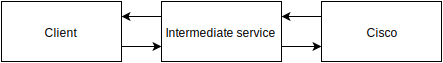
\includegraphics[scale=0.9]{graphics/cisco_usage.png}
	\caption{Cisco usage}
	\label{fig:cisco_usage}
	\end{center} 
\end{figure}

A Restful service typically communicates using the HTTP or HTTPS protocols, and functions by receiving requests on specific URIs to which it responds in a predefined way. As an example we can send a HTTPS GET request to 64.103.26.61 with the URI "/api/contextaware/v1/location/clients" and, given that we supply the correct user name and password, receive a string of data corresponding to the type of request. \sfx{kilde}

To create a transparent Restful service that duplicates the functionality of the Cisco Restful API, we need to make use of the same URIs as the Cisco API\sfx{link to cisco api}. This is done with the use of the Jersey Java library, which affords the possibility of creating a HTTP server and specifying what URIs can be requested.

\begin{lstlisting}[caption={Adding a URI},label={lst:context_code},language=inc_Java]
server.createContext("/api/contextaware/v1/location/clients", httpExchange -> {
            if (VerifyConnection(httpExchange) == false){
                return;
            }

            String response = CollectAllClients(username, password, ciscoIp);
            httpExchange.sendResponseHeaders(200, response.length());
            OutputStream os = httpExchange.getResponseBody();
            os.write(response.getBytes(Charset.forName("UTF-8")));
            os.close();
        });
\end{lstlisting}
The code example shown on \cref{lst:context_code} shows how this is done. The createContext method takes two parameters: a string for the URI and an anonymous function implementing an interface. The anonymous function decides what actions are performed once a connection is established, in this case some verification is performed immediately to authenticate the user. A response is generated based on the URI; on line 4 we retrieve all clients from Cisco, which is then written though an OutputStream to the requester. 

In order to accommodate the privacy concern, we implement some simple methods to obfuscate mac-address and user name. 

\section{Sprint evaluation}
To conclude on the first sprint, we have explored different methods and technologies to perform indoor positioning. Furthermore we have described certain issues related to person sensitive data, and finally we developed an initial design of a RESTful service to operate as an intermediate service for Cisco MSE. 

As such the goals for the first sprint have been fulfilled.